% Synthetic validation corpus for image-OCR classification and recognition.
%
% Purpose: exercise the whole real pipeline -- pdflatex -> PDF -> pymupdf4llm crop extraction ->
% classification -> OCR -- on content whose ground truth is known, without shipping anyone's
% actual library. Every element carries a CORPUSMARK token in the prose immediately before it,
% which lands in the extracted text layer and therefore in a crop's `text_before`. That is how
% an observed crop is tied back to the element that produced it; nothing depends on crop
% ordering or on filenames.
%
% Positive examples are elements whose content must be recovered. Negative examples are page
% furniture that must never be sent to an OCR model. The negatives are chosen adversarially: a
% full-width decorative rule is wide and short, exactly the shape of a display equation, so a
% classifier keyed on aspect ratio alone will get it wrong.
%
% Rebuild with: python tools/build_ocr_corpus.py

\documentclass[11pt,a4paper]{article}
\usepackage{amsmath,amssymb}
\usepackage{booktabs}
\usepackage{xcolor}
\usepackage{graphicx}
\usepackage{tikz}
\usepackage{pgfplots}
\pgfplotsset{compat=1.16}
\usetikzlibrary{matrix,positioning,arrows.meta,shapes.geometric}
\usepackage[margin=2.5cm]{geometry}
\pagestyle{plain}

\begin{document}

\section*{Synthetic OCR Validation Corpus}

This document exists to be converted, not read. Prose paragraphs are present so that crops have
neighbouring text to be located by, mirroring how a real article reads around its display
elements.

% ---------------------------------------------------------------- positive: equations

CORPUSMARK-EQ-001 A numbered display equation, the standard weighted arithmetic mean:
\begin{equation}
\bar{x}_{w} = \frac{\sum_{i=1}^{n} w_i\, x_i}{\sum_{i=1}^{n} w_i}
\end{equation}
The weights are normalised so that the result stays bounded.

CORPUSMARK-EQ-002 A fraction combined with an improper integral:
\begin{equation}
\frac{\partial u}{\partial t} = \int_{0}^{\infty} e^{-\lambda t}\, d\mu(\lambda)
\end{equation}
This form appears throughout the transform literature.

CORPUSMARK-EQ-003 Nested subscripts and superscripts:
\begin{equation}
\sigma^{2}_{i,j} = \frac{1}{N-1}\sum_{k=1}^{N}\left(x_{k}^{(i)} - \bar{x}^{(i)}\right)^{2}
\end{equation}
Sample variance, written the long way.

CORPUSMARK-EQ-004 A multi-line aligned derivation, which occupies several rows and is therefore
much taller than a single-line equation:
\begin{align}
f(x) &= (x+1)^{2} \\
     &= x^{2} + 2x + 1 \\
     &= x^{2} + 2x + 1 + 0
\end{align}
Each step follows from the previous one.

CORPUSMARK-EQ-005 A matrix, which is tall relative to its width:
\begin{equation}
A = \begin{pmatrix}
a_{11} & a_{12} & a_{13} \\
a_{21} & a_{22} & a_{23} \\
a_{31} & a_{32} & a_{33}
\end{pmatrix}
\end{equation}
Matrices are the classic case where a wide-and-short assumption fails.

CORPUSMARK-EQ-006 A piecewise definition:
\begin{equation}
H(x) = \begin{cases}
0 & \text{if } x < 0 \\
1 & \text{if } x \geq 0
\end{cases}
\end{equation}
The Heaviside step, defined by cases.

CORPUSMARK-EQ-007 Set-theoretic and logical operators, which rely on symbol fonts:
\begin{equation}
\forall \varepsilon > 0\ \exists \delta > 0 : |x - a| < \delta \implies |f(x) - f(a)| < \varepsilon
\end{equation}
The usual definition of continuity.

CORPUSMARK-EQ-008 Greek letters mixed with relations:
\begin{equation}
\alpha \wedge \beta \subseteq \Gamma \cup \Delta, \qquad \theta \in \Theta \setminus \{\emptyset\}
\end{equation}
Symbols here span several Unicode blocks.

CORPUSMARK-EQ-009 An unnumbered display equation:
\[
\lim_{n \to \infty} \left(1 + \frac{1}{n}\right)^{n} = e
\]
Unnumbered forms are common in proofs.

CORPUSMARK-EQ-010 An equation carrying units and upright text:
\begin{equation}
E_{\text{total}} = mc^{2} + \tfrac{1}{2}mv^{2} \quad [\mathrm{J}]
\end{equation}
Mixed italic and upright content in one expression.

CORPUSMARK-EQ-011 A display equation with an embedded natural-language phrase, which the model
must reproduce as words rather than garble into symbols:
\begin{equation}
g(x) \geq 0 \quad \text{for all } x \in \mathbb{R}, \qquad \text{and } g(0) = 0.
\end{equation}
Text inside mathematics is a distinct recognition case from surrounding prose.

CORPUSMARK-EQ-012 The next display equation is introduced by a table cross-reference in running
prose. The sentence begins with a table label but is not a caption for the equation, and the
equation is a wide single-line strip -- the exact shape that was being mislabelled as a table.

Table 3 reports the fitted coefficients of the following linear predictor:
\begin{equation}
\hat{y} = \beta_{0} + \beta_{1} x_{1} + \beta_{2} x_{2} + \beta_{3} x_{3} + \varepsilon
\end{equation}
The residual term is assumed to be mean zero.

CORPUSMARK-EQ-013 The next display equation is introduced by a figure cross-reference sentence,
the analogous trap for figures rather than tables.

Figure 4 shows that the estimator can be written in the closed form
\begin{equation}
\hat{\theta} = \left( X^{\top} X \right)^{-1} X^{\top} y
\end{equation}
which is the ordinary least squares solution.

CORPUSMARK-EQ-014 A norm and inner product:
\begin{equation}
\lVert x \rVert_{2}^{2} = \langle x, x \rangle = \sum_{i=1}^{d} x_{i}^{2}
\end{equation}
Vector norms recur throughout the optimisation literature.

CORPUSMARK-EQ-015 A binomial coefficient expanded as a product:
\begin{equation}
\binom{n}{k} = \frac{n!}{k!\,(n-k)!} = \prod_{i=1}^{k} \frac{n - i + 1}{i}
\end{equation}
Combinatorial identities stress factorial and product notation.

CORPUSMARK-EQ-016 A nested radical with a closed form:
\begin{equation}
\sqrt{a + \sqrt{a + \sqrt{a + \cdots}}} = \frac{1 + \sqrt{1 + 4a}}{2}
\end{equation}
Nested radicals produce deeply stacked glyphs.

CORPUSMARK-EQBLOCK-001 A block of several short stacked equations whose bounding box is close to
square, the shape that geometry misreads as a figure rather than mathematics:
\begin{equation}
\begin{aligned}
Y_{1} &= X_{1} \\
Y_{2} &= X_{1} + X_{2} \\
Y_{3} &= X_{1} + X_{2} + X_{3} \\
Y_{4} &= X_{1} + X_{2} + X_{3} + X_{4}
\end{aligned}
\end{equation}
A cumulative construction, one term added per line.

CORPUSMARK-EQBOX-001 A display equation set inside a shaded definition box, the way a textbook
frames a key formula. The shading makes the whole region a graphic, and the words must be kept:
\begin{center}
\colorbox{black!10}{\parbox{0.75\linewidth}{\centering
\textbf{Definition:}\\[1mm]
$\displaystyle F = \frac{MS_{\text{between}}}{MS_{\text{within}}}$\\[1mm]
with $df_{\text{between}} = p - 1$ and $df_{\text{within}} = N - p$.}}
\end{center}
The boxed form recurs wherever a definition is highlighted.

% ---------------------------------------------------------------- negative: inline math

CORPUSMARK-INLINE-001 Inline mathematics stays in the text layer and must not become a crop:
the identity $e^{i\pi} + 1 = 0$ and the bound $0 \leq p \leq 1$ both sit inside this running
sentence, alongside symbols such as $\alpha$, $\beta$ and $\sum_{i} x_i$, none of which the
extractor pulls out into an image.

% ---------------------------------------------------------------- positive: table

CORPUSMARK-TBL-001 A ruled numeric table:

\begin{center}
\begin{tabular}{lrr}
\toprule
Condition & Mean & SD \\
\midrule
Baseline  & 12.40 & 1.15 \\
Treatment & 15.82 & 1.640 \\
Control   & 12.11 & 1.09 \\
\bottomrule
\end{tabular}
\end{center}

The table above reports descriptive statistics.

% ---------------------------------------------------------------- positive: figure

CORPUSMARK-FIG-001 A vector figure drawn from primitives, with a caption beneath it:

\begin{center}
\setlength{\unitlength}{1mm}
\begin{picture}(60,35)
  \put(0,0){\line(1,0){60}}
  \put(0,0){\line(0,1){35}}
  \put(0,0){\line(3,2){45}}
  \put(0,5){\line(2,1){50}}
  \put(0,12){\line(4,1){55}}
  \put(10,28){\circle*{2}}
  \put(25,20){\circle*{2}}
  \put(40,30){\circle*{2}}
\end{picture}
\end{center}

\noindent\textbf{Fig. 1} Line segments and plotted points, captioned in the style a converted
article uses.

CORPUSMARK-FIG-002 A bar chart of a discrete probability distribution, the commonest figure in a
statistics text:

\begin{center}
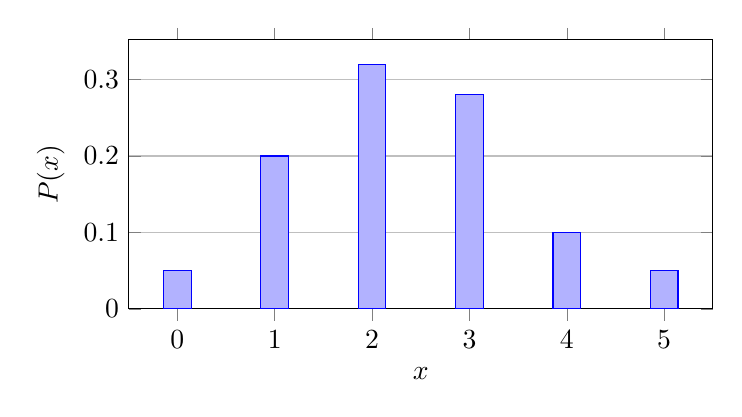
\begin{tikzpicture}
\begin{axis}[ybar, bar width=10pt, width=9cm, height=5cm, ymin=0, xlabel={$x$},
             ylabel={$P(x)$}, xtick=data, ymajorgrids]
\addplot coordinates {(0,0.05) (1,0.20) (2,0.32) (3,0.28) (4,0.10) (5,0.05)};
\end{axis}
\end{tikzpicture}
\end{center}

\noindent\textbf{Fig. 2} A probability mass function.

CORPUSMARK-FIG-003 A normal density curve with two shaded tail regions, exactly the figure a text
uses to introduce significance testing:

\begin{center}
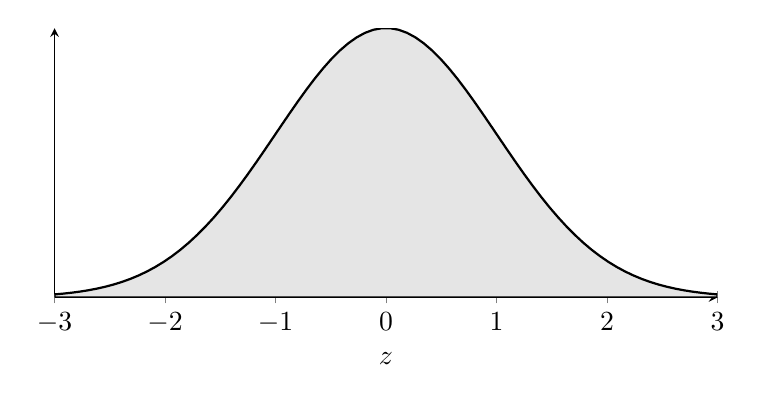
\begin{tikzpicture}
\begin{axis}[width=10cm, height=5cm, ymin=0, axis lines=left, xlabel={$z$}, ytick=\empty,
             samples=80, domain=-3:3]
\addplot[thick, fill=gray!20] {exp(-x^2/2)/sqrt(2*pi)} \closedcycle;
\end{axis}
\end{tikzpicture}
\end{center}

\noindent\textbf{Fig. 3} The standard normal density.

CORPUSMARK-FIG-004 A line plot drawn on a full coordinate grid. The grid lines are the trap: a
classifier can mistake the ruled background for a table.

\begin{center}
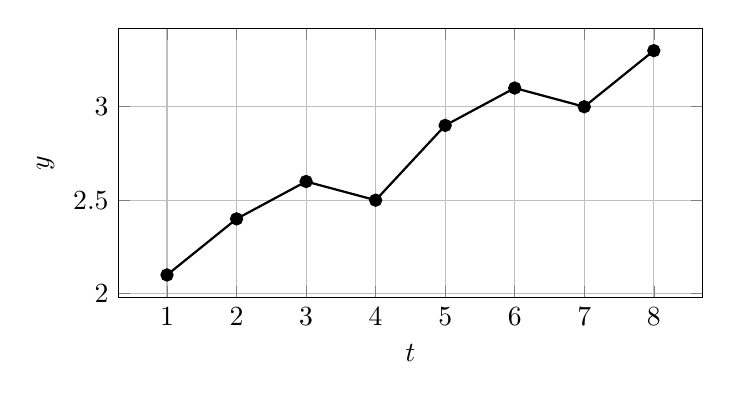
\begin{tikzpicture}
\begin{axis}[width=9cm, height=5cm, grid=both, xlabel={$t$}, ylabel={$y$}]
\addplot[thick, mark=*] coordinates {(1,2.1)(2,2.4)(3,2.6)(4,2.5)(5,2.9)(6,3.1)(7,3.0)(8,3.3)};
\end{axis}
\end{tikzpicture}
\end{center}

\noindent\textbf{Fig. 4} A response curve on a grid.

CORPUSMARK-FIG-005 A Venn diagram of two overlapping events inside a sample space:

\begin{center}
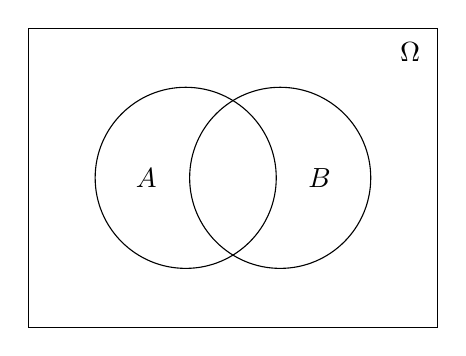
\begin{tikzpicture}
\draw (-2.6,-1.9) rectangle (2.6,1.9);
\node at (2.25,1.6) {$\Omega$};
\draw (-0.6,0) circle (1.15cm);
\draw (0.6,0) circle (1.15cm);
\node at (-1.1,0) {$A$};
\node at (1.1,0) {$B$};
\end{tikzpicture}
\end{center}

\noindent\textbf{Fig. 5} Two events and their intersection.

CORPUSMARK-FIG-006 A path diagram with a latent variable and its indicators, the schematic a
structural-equation-modelling paper prints:

\begin{center}
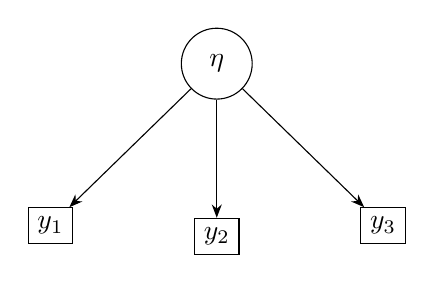
\begin{tikzpicture}[>=Stealth, node distance=1.5cm and 1.5cm]
\node[ellipse, draw, minimum size=0.9cm] (eta) {$\eta$};
\node[rectangle, draw, below left=of eta] (y1) {$y_1$};
\node[rectangle, draw, below=of eta] (y2) {$y_2$};
\node[rectangle, draw, below right=of eta] (y3) {$y_3$};
\draw[->] (eta) -- (y1);
\draw[->] (eta) -- (y2);
\draw[->] (eta) -- (y3);
\end{tikzpicture}
\end{center}

\noindent\textbf{Fig. 6} A one-factor measurement model.

% ---------------------------------------------------------------- positive: table CROPS
% Drawn as TikZ graphics, not tabular environments: pymupdf4llm converts a `tabular` to Markdown
% text (no crop), but rasterises a drawn graphic. This is the only way to synthesise a table CROP,
% which is the failure mode a real library hits when a publisher's table defeats the text extractor.

CORPUSMARK-TBL-002 A contingency table embedded as a raster image built by the corpus tool. A
raster table has no text layer, so -- unlike a LaTeX tabular -- it is extracted as an image crop,
reproducing the real failure mode where a publisher's table defeats the text extractor:

\begin{center}
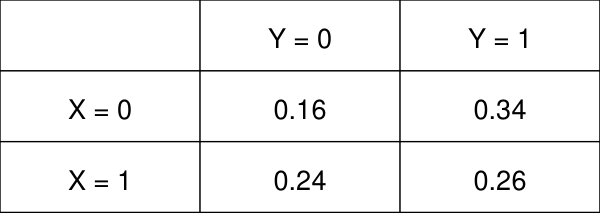
\includegraphics[width=6cm]{table_contingency.png}
\end{center}

\noindent\textbf{Tab. 2} A joint probability table.

CORPUSMARK-TBL-003 A denser computational table of fractions, also embedded as a raster image. A
wall of fractions like this is easily misread as a single large equation:

\begin{center}
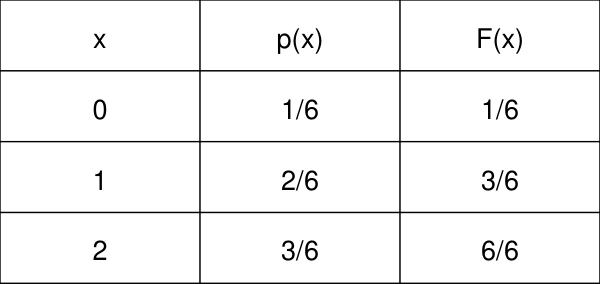
\includegraphics[width=6.5cm]{table_computational.png}
\end{center}

\noindent\textbf{Tab. 3} A cumulative distribution, tabulated.

% ---------------------------------------------------------------- negative: page furniture

CORPUSMARK-NEG-001 A full-width decorative band follows. It is wide and short -- the same shape
as a display equation, and the reason a classifier keyed on aspect ratio alone fails -- and it
contains nothing to read:

\noindent\textcolor{orange}{\rule{\linewidth}{7mm}}

That band carries no content.

CORPUSMARK-NEG-002 A narrow vertical spine bar follows, of the kind publishers print down a
page edge:

\noindent\textcolor{orange}{\rule{12mm}{130mm}}

That bar carries no content either.

CORPUSMARK-NEG-003 A solid square block, standing in for a logo or a masthead device:

\noindent\textcolor{black!70}{\rule{22mm}{22mm}}

Blocks like this are pure decoration.

CORPUSMARK-NEG-004 A separator band of two thick rules, wide and short like the first negative:

\noindent\textcolor{black!30}{\rule{\linewidth}{4mm}}\\[2mm]
\noindent\textcolor{black!30}{\rule{\linewidth}{4mm}}

Nothing above this line needs recognising.

CORPUSMARK-DEC-001 A small empty framed box, the shape an extracted form-field or checkbox glyph
takes -- content-free, and small enough that a size gate should drop it before any model sees it:

\begin{center}

\begin{tikzpicture}
\draw[line width=0.6pt] (0,0) rectangle (0.5,0.45);
\end{tikzpicture}
\end{center}

An empty box carries nothing to recognise.

CORPUSMARK-DEC-002 A vertical gradient bar, the decorative device a publisher runs down a column.
It is a graphic with no text, and must never be sent to an OCR model as a formula:

\begin{center}

\begin{tikzpicture}
\shade[top color=blue!70, bottom color=blue!5] (0,0) rectangle (0.4,3.2);
\end{tikzpicture}
\end{center}

The bar is pure decoration.

\end{document}
